\RequirePackage[orthodox]{nag}
\documentclass[11pt]{article}

%% Define the include path
\makeatletter
\providecommand*{\input@path}{}
\g@addto@macro\input@path{{include/}{../include/}}
\makeatother

\usepackage{../../include/akazachk}

\title{ECH4905 ChemE Optimization HW 2}
\author{Andres Espinosa}

\begin{document}
\maketitle

\section{Problem 1}
Write the following problem in standard form
\begin{align}
  \text{maximize} & \quad 3 x_1 + 2x_2 \\
  \text{subject to} & \quad -2x_1 + x_2 \geq 1 \\
  & \quad x_1 + 3x_2 = 2
\end{align}
\\
\textbf{Solution: }
% TODO: SOLVE PROBLEM
\begin{align}
  \text{minimize} & \quad -3 x_1 - 2x_2 \\
  \text{subject to} & \quad  \\
  & \quad 
\end{align}

\section{Problem 2}
An engineering factory makes seven products on the following machines: four
grinders, two vertical drills, three horizontal drills, one borer and one planer. Each product
yields a certain contribution to profit (defined in dollars per unit). These quantities together
with the unit production times required on each process are given below.

\begin{table}[h!]
\centering
\begin{tabular}{|c|c|c|c|c|c|c|c|}
\hline
 & P1 & P2 & P3 & P4 & P5 & P6 & P7 \\
\hline
Contribution to profit & 10 & 6 & 8 & 4 & 11 & 9 & 3 \\
\hline
Grinding (hours) & 0.5 & 0.7 & - & - & 0.3 & 0.2 & 0.5 \\
\hline
Vertical drilling (hours) & 0.1 & 0.2 & - & 0.3 & - & 0.6 & - \\
\hline
Horizontal drilling (hours) & 0.2 & - & 0.8 & - & - & - & 0.6 \\
\hline
Boring (hours) & 0.05 & 0.03 & - & 0.07 & 0.1 & - & 0.08 \\
\hline
Planning (hours) & - & - & 0.01 & - & 0.05 & - & 0.05 \\
\hline
Demand (units) & 500 & 1000 & 300 & 300 & 800 & 200 & 100 \\
\hline
\end{tabular}
\caption{Production data for the engineering factory}
\label{tab_problem2}
\end{table}

There are some marketing limitations to the production (demand), these are given as the bottom row in table \ref{tab_problem2}.
We can assume that the factory works 24 days, and that each day each machine works for
16 hours.
Formulate an LP to find the optimal product distribution.
\\
\textbf{Solution: }
% TODO: SOLVE PROBLEM

\section{Problem 3}
Solve problem 2 but consider that the demand of each product is a function of
the month, i.e., that the demand for product $i$ in month $m$ is given by parameter $d_{i,m}$. In this
case, assume that you can store a maximum amount of 100 units of product each month at
a cost of 0.5/unit-month. At the beginning of the planning period there is no inventory, but at
the end we want to have 50 units of each product in storage.

When and what should the factory produce to maximize profit?
\\
\textbf{Solution: }
% TODO: SOLVE PROBLEM

\section{Problem 4}
Formulate a LP model for the following reaction network (image \ref{fig:problem_4_rn}), assuming that you want
to maximize the production rate of 3-methyltetrahydrofuran, and that you have an incoming
flux of itaconic acid equal to 1. For the sake of simplicity you can ignore the water and
hydrogen that would be required to balance the equations.
\begin{figure}[htbp]
  \centerline{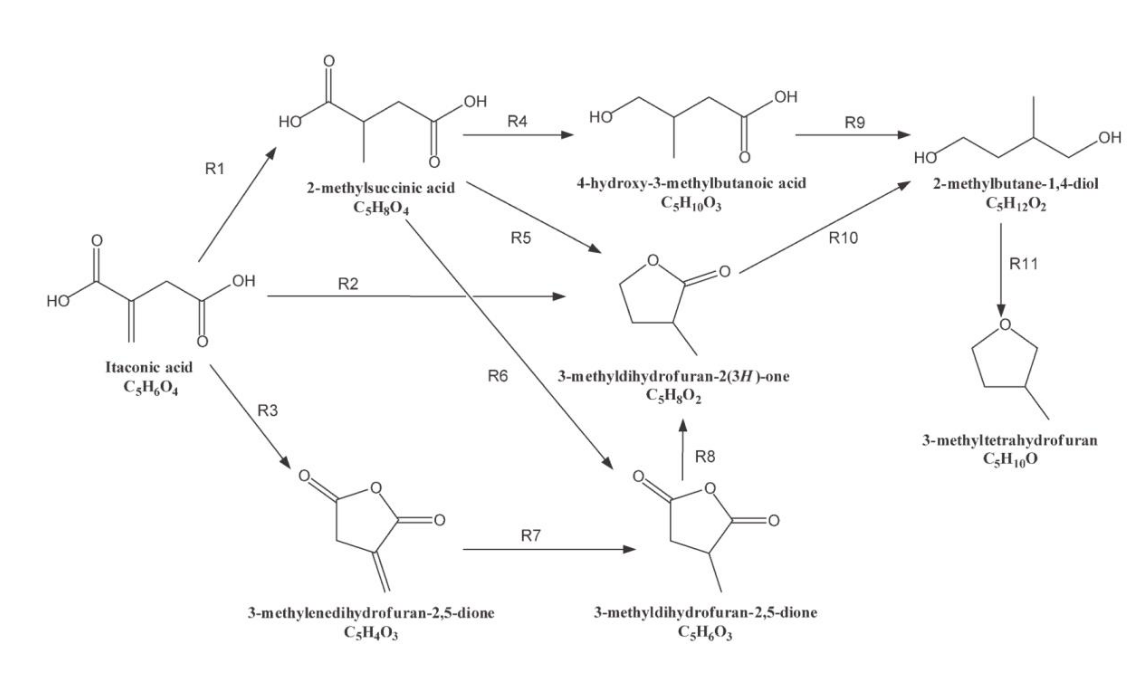
\includegraphics[width=0.75\textwidth]{images/image.png}}
  \caption{Problem 4 Reaction Network}
  \label{fig:problem_4_rn}
\end{figure}

\textbf{Solution: }
% TODO: SOLVE PROBLEM


\end{document}